\section{$S=1$ Thermometry}
Again for $S=1$ we will consider a divacancy which have zero-
field splitting (ZFS) frequencies are at approximately
$D = 1.365$ GHz \cite{Falk2013}.

For this application we will need every term in \eqref{eq:total_hamiltonian} as $D$ is affected by $\vec{B}$, $\vec{E}$, temperature, and pressure \cite{Fujiwara2021}. We will reduce the constant terms as we did in \ref{s1_magnetometry}

\begin{equation}
	\begin{align}
		H & = g \mu_B \hat{\vec{S}}\cdot \vec{B} +
		D(\hat{S}_z^2)  + E(\hat{S}_x^2 - \hat{S}_y^2) \\
		  & +d_\parallel E_z(\hat{S}_z^2)
		- d_\perp  E_y(\hat{S}_x^2 - \hat{S}_y^2   ) + d_\perp E_x(\hat{S}_x\hat{S}_y + \hat{S}_y\hat{S}_x).
	\end{align}
	\tag{\ref{eq:total_hamiltonian}}
\end{equation}

In this discussion we will consider the pressure to be constant, but as we will describe at the end of this section, by holding temperature constant the same scheme could be used to detect pressure.

There are two main approaches to thermometry:
\begin{description}
	\item[ZFS Temperature Dependence.] The ZFS $D$ may, depending on the specific spin system being studies, be sensitive to changes in temperature, which will be exploited in this section.
    \item[Photoluminescence.] The photoluminescence of the spin system may have a dependence on temperature, which we will exploit in section \ref{spin1.5-thermo}.
\end{description}

We will exploit the temperature dependence of ZFS $D$ which results
from thermal lattice expansion and a temperature dependence of the electron–phonon interaction \cite{PhysRevB.90.235205,PhysRevB.90.041201}. We will also consider the influences of $\vec{B}$ and $\vec{E}$ to be well known, this could be achieved by careful experiment design or by measurement. We will therefore assume they may be disregarded in this discussion with the exception of a well known $\vec{B}$ field applied along the defect axis.

This allows us to reduce our Hamiltonian down to only
\begin{equation}
	H' = D(T) \hat{S}_z^2
	\label{eq:}
\end{equation}
which when we substitute our spin operator \eqref{eq:s1_spin_operators} we find
\begin{equation}
	H' = \begin{pmatrix}
		D(T) & 0 & 0    \\
		0    & 0 & 0    \\
		0    & 0 & D(T)
	\end{pmatrix}.
	\label{eq:s1_thermometry_matrix}
\end{equation}

We see from \eqref{eq:s1_thermometry_matrix} that the $m_s = \pm 1$ states are both uniformly affected by the temperature dependence of $D$ while the $m_s =0$ state is not influenced by the change. Therefore, the $\Delta m_s = \pm1$ transitions, detectable in EPR, are affected.

The temperature dependence of $D$ is visualised as a magnetic field is applied along the defect axis in figure \ref{fig:s1-temp-dependence}.

\begin{figure}[H]
	\begin{center}
		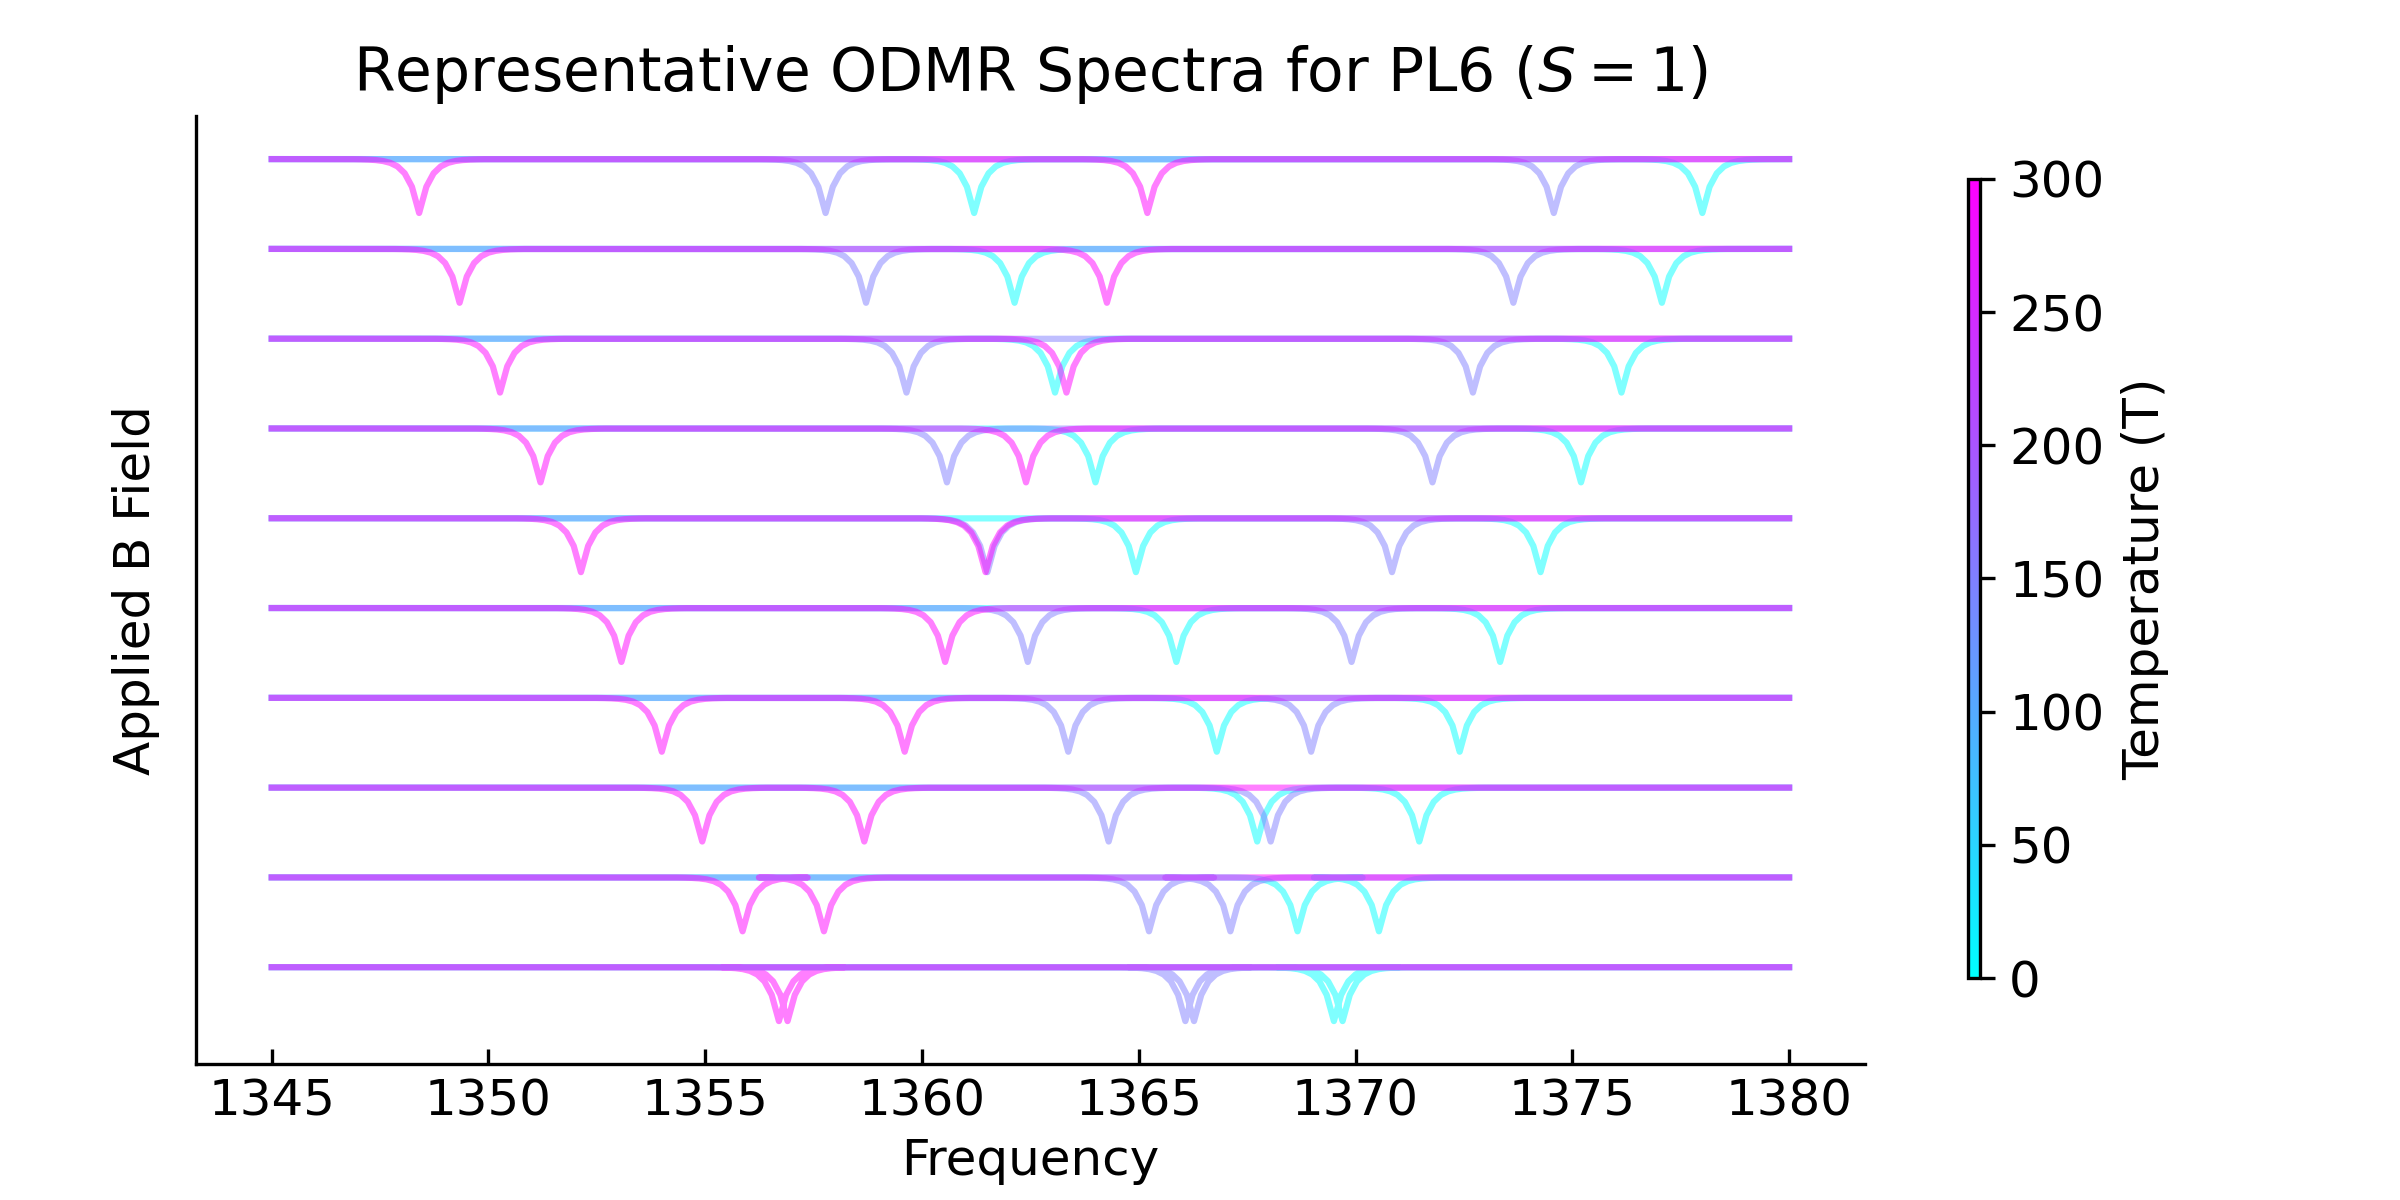
\includegraphics[width=0.95\textwidth]{figures/ODMR-s1-temp-dependence.png}
	\end{center}
	\caption{}\label{fig:s1-temp-dependence}
\end{figure}

For any $B > 0$, since the Zeeman effect acts on the $m_s = \pm1$ states symmetrically we may find $D$ using
\begin{equation}
	f_1 = D(T) + \gamma B, \quad f_2 = D(T) - \gamma B
	\label{eq:}
\end{equation}
and computing $D(T)$
\begin{equation}
	D(T) = \frac{f_1 + f_2}{2}.
	\label{eq:average_freq_thermo}
\end{equation}

The temperature dependence of $D$ has been studied for both PL5 and PL6 \cite{,}. The PL6 dependence may be fit to the Debye-model formula \cite{Plakhotnik2014}, Varshni-form formula \cite{Li2017} or a polynomial-form formula \cite{PhysRevB.104.125305, Yan2018}

\begin{equation}
	\begin{align}
		D(T) & = 1364.6 + 3.5 \times 10^{-3}T - 1.8\times10^{-4}T^2                              \\
		     & - 1.5 \times 10^{-7}T^3 + 1.6 \times 10^{-9}T^4 - 2.7 × 10^{-12}T^5  \text{ MHz}.
	\end{align}
	\label{eq:PL6-temp-polynomial}
\end{equation}

Any of the fits may be used to infer temperature from the measured value of $D$.


% \cite{Chen2011}
% \cite{ajev2009}

% Example
% \cite{Quan:23}

% \todo[inline]{Distribute references properly}
%
%
% We can use spin defects in SiC for temperature sensing.
% This work will focus on the first method of thermometry, the dependence of $D$ on temperature is discussed in section \ref{D_vs_temp}. Unlike $\vec{B}$ and $\vec{E}$ field sensing, there is no direction associated with temperature so the sensing regime may be simpler.
%
% In the simplest case thermometry is then achieved in the presence of a well known applied magnetic field.
%
% The measurement stems from the change of the value of
% D mapped into the change of the oscillation frequency of the
% relative variation of the photoluminescence intensity induced by the microwave pulse sequence.
%
% Since the degeneracy is raised symmetrically, the value of $D$ is the average of the two resonant frequencies. The value of $D$ can then be mapped to a temperature.
%
% This is visualised in figure \ref{fig:pl6-3temps}.
%
% \begin{figure}[h]
%     \begin{center}
%         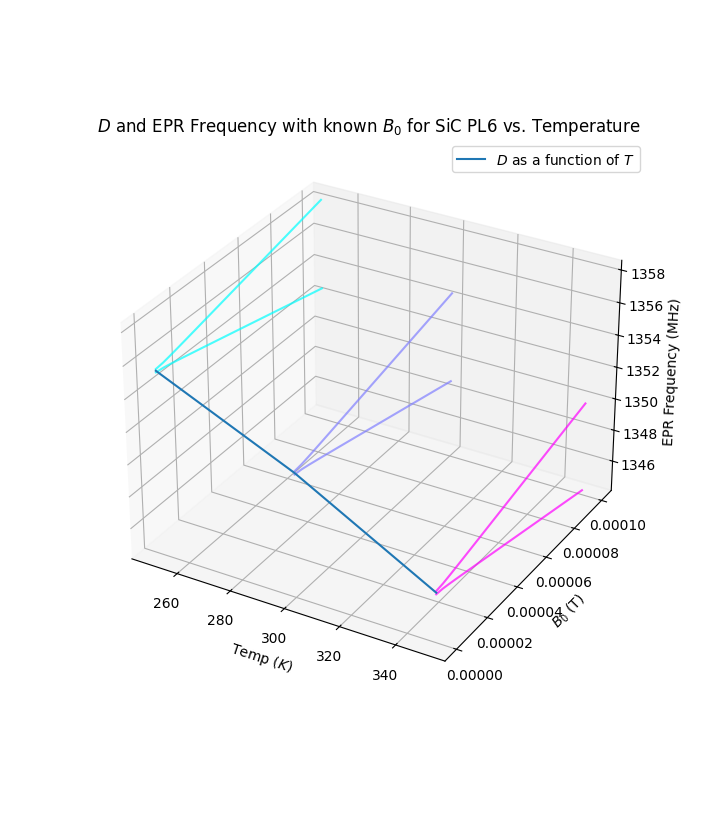
\includegraphics[width=0.8\textwidth]{figures/PL6-DvsT-3temps.png}
%     \end{center}
%     \caption{\td{write caption}}\label{fig:pl6-3temps}
% \end{figure}


\begin{summary}{$S=1$ Thermometry Summary}{sum:spin1thermo}
	We may achieve thermometry using a $S=1$ system provided:
	\begin{enumerate}
		\item The influence of $\vec{B}, \vec{E}$ and pressure are well known.
		\item The temperature dependence of the defect has been studied and fit to an equation e.g.
		      \begin{equation}
			      \tcbhighmath{
                      \begin{align}
				      D(T) & = 1364.6 + 3.5 \times 10^{-3}T - 1.8\times10^{-4}T^2                              \\
				      & - 1.5 \times 10^{-7}T^3 + 1.6 \times 10^{-9}T^4 - 2.7 × 10^{-12}T^5  \text{ MHz}.
                      \end{align}
			      }
			      \tag{\ref{eq:PL6-temp-polynomial}}
		      \end{equation}

		\item We can resolve \textbf{one frequency} (in zero field) or \textbf{two frequencies} if the $m_s = \pm1$ degeneracy has been lifted corresponding to the defect in the CW-ODMR spectra. This may be used to find $D$ e.g. with $B\parallel z$ we have
		      \begin{equation}
			      \tcbhighmath{
				      D(T) = \frac{f_1 + f_2}{2}
			      }
			      \tag{\ref{eq:average_freq_thermo}}
		      \end{equation}

	\end{enumerate}
\end{summary}

The methods described in this section have exploited the change of ZFS $D$ due to temperature, which is characteristically the same as the change due to pressure. The scheme may therefore be used for sensing pressure as well as sensing temperature.

